\documentclass[letterpaper,man,natbib]{apa6}  %Leave this stuff alone

\usepackage[english]{babel}
\usepackage[utf8x]{inputenc}
\usepackage{amsmath}
\usepackage{graphicx}
\usepackage{booktabs}
\usepackage[export]{adjustbox}

% override apa6 section headers
% https://tex.stackexchange.com/questions/125537/how-to-modify-subsubsection-header-apa6-cls
\makeatletter
\renewcommand{\subsubsection}{\@startsection{subsubsection}{3}
  {\z@}%
  {\b@level@two@skip}{\e@level@two@skip}%
  {\normalfont\normalsize\bfseries}}
\makeatother

% dashed line (https://tex.stackexchange.com/questions/112343/beautiful-table-samples)
\usepackage{array}
\usepackage{arydshln}
\setlength\dashlinedash{0.2pt}
\setlength\dashlinegap{1.5pt}
\setlength\arrayrulewidth{0.3pt}

\title{The MACE is essentially unidimensional: Bifactor models of the `Maltreatment and Abuse Chronology of Exposure' scale}
\shorttitle{Bifactor models of MACE}
\author{Samuel Zorowitz$^1$, Lauri Tuominen$^{2}$}
\affiliation{$^1$Princeton Neuroscience Institute, Princeton University, USA\\$^2$The Royal’s Institute of Mental Health Research, University of Ottawa, Canada}

\abstract{Your abstract here.}

\begin{document}

\maketitle

\section{Introduction}

Childhood maltreatment is an unfortunately common experience for children across the globe \citep{stoltenborgh2015prevalence}. It is a risk factor for multiple poor outcomes later in life, including the onset of mental illness \citep{macmillan2001childhood, green2010childhood, kessler2010childhood}, challenges in cognitive functioning \citep{kavanaugh2017neurocognitive, r2018common, su2019does}, and poorer physical health \citep{wegman2009meta, widom2012prospective, goodwin2004association}. Childhood maltreatment also predicts worse treatment outcomes for many psychiatric disorders \citep{nanni2012childhood, thomas2019childhood, schuckher2019history}. Thus, the reliable and valid assessment of childhood maltreatment is an important research goal in order to refine our understanding of the link between maltreatment and health outcomes; augment treatment strategies for victims of childhood maltreatment; and ultimately design better interventions to prevent maltreatment in the first place. 

There already exist many measures of childhood abuse and maltreatment for researchers to choose from \citep{saini2019systematic}. One recently developed measure, the Maltreatment and Abuse Chronology of Exposure (MACE) scale \citep{teicher2015maltreatment}, has a number of notable advantages. The MACE is a 52-item retrospective self-report questionnaire comprised of 10 short subscales that each assess a unique type of childhood maltreatment. Six of these (e.g. parental verbal abuse, physical abuse, nonverbal emotional abuse, sexual abuse, emotional neglect, physical neglect) overlap with other common measures of abuse; the remaining four assess forms of maltreatment that are less frequently represented in other measures (e.g. peer victimization, witnessing domestic violence). The items in the MACE were carefully selected to measure adverse childhood experiences of increasing severity in order to more finely differentiate people of varying exposure levels. The MACE also measures the timing of maltreatment experiences, which is critical for investigating how the onset and duration of abuse shapes trajectories of development. The MACE provides two measures, an overall severity score (number of maltreatment experiences) and a multiplicity score (number of types of maltreatment experienced), with excellent temporal stability, good convergent validity with other standard measures, and improved predictive validity in predicting psychiatric symptom ratings \citep{teicher2015maltreatment}. For these reasons, the MACE has been listed as among the best measures of childhood maltreatment currently available \citep{saini2019systematic, georgieva2022systematic}.

In recent years, there have been calls for childhood maltreatment research to move away from the cumulative risk framework \citep{evans2013cumulative} --- which focuses only on the number of adverse experiences --- towards a dimensional approach, which emphasizes how distinct types of maltreatment uniquely shape developmental trajectories \citep{mclaughlin2016beyond, belsky2012beyond}. In response, some researchers have begun to use the MACE to form new indices of maltreatment in lieu of or in addition to the severity and multiplicity scores. For example, some have investigated the unique contributions of individual differences on all 10 MACE subscale scores to the development of psychopathology \citep{schalinski2015type, gerke2018childhood, schalinski2019early}. Following a prominent dimensional model of maltreatment \citep{mclaughlin2014childhood}, other groups have made composite indices of threat and deprivation experiences using items in the MACE that respectively assess abuse and neglect experiences \citep{schalinski2018defining, schalinski2019environmental, teicher2018differential}. Though these alternatives maltreatment scores may yield new insight, their psychometric properties have not been extensively investigated.   

One critical challenge in measuring childhood maltreatment is the high co-occurrence adverse experiences. That is, children experiencing one form of maltreatment (e.g. physical abuse) are likely to experience one or more other types (e.g. emotional abuse; \citealt{green2010childhood, mclaughlin2012childhood, marques2021risk, mersky2017rethinking}). As a consequence, isolating the unique contribution of one type of maltreatment to the development of some negative outcome is difficult insofar as any one type of adversity is likely confounded with general maltreatment. Concretely, this means that researchers who want to study the effects of particular types of maltreatment using subscale scores or composite indices need to verify those measures reflect a construct mostly independent of overall maltreatment, lest they draw spurious conclusions.

Bifactor models, one type of hierarchical factor models, are well-suited for addressing this issue \citep{bornovalova2020appropriate}. They assume that the covariance structure of a set of items can be accounted for by a general factor, reflecting shared variance across all items, and one or more specific factors, reflecting additional shared variance among subsets of items \citep{Reise2012-ql}. Crucially, bifactor models can be used to calculate model-based reliability statistics, including the omega hierarchical ($\omega_h$) and omega subscale ($\omega_s$) indices, which respectively measure the proportion of variance in total and subscale scores attributable to the general factor and specific factors \citep{reise2013applying, rodriguez2016evaluating}. Applied to the MACE scale, these indices can inform researchers as to whether subscale scores or composite indices for particular types of maltreatment are interpretable as such, or if they instead predominantly reflect overall maltreatment. 

% summary of paper paragraph tk

\section{Methods}

\subsection{Participants}

The participants in the current study (N=1633 total) belonged to one of two samples. The first sample of participants (N=1051) are from the original development of the MACE scale \citep{teicher2015maltreatment}. The full recruitment details for this sample have been reported elsewhere \citep{teicher2015maltreatment}. Briefly, these participants were recruited from the greater Boston area between 2010 and 2013. Inclusion criteria included being medically healthy, unmedicated, and between 18–25 years of age.  This sample will hereafter be referred to as the \textit{original} sample. 

The second sample of participants (N=687) were recruited from the Prolific Academic platform (\url{https://www.prolific.co}) to participate in an online experiment in August -- October, 2021. Of these, N=582 were retained for analysis (see Exclusion Criteria below). Participants were eligible for participation if they were 18 years or older and currently resided in the United States or Canada. Participants received monetary compensation for their time (rate: \$12 USD/hr). This study was approved by the Institutional Review Board of the University of Ottawa (\#2021003), and all participants provided informed consent. This sample will hereafter be referred to as the \textit{replication} sample. 

In both the original and replication samples, the majority of participants identified as women (original: male = 381, female = 670; replication: male = 258, female = 310, nonbinary or other = 9, rather not say = 5). The original sample is comprised of proportionally more woman than the replication sample ($z = 4.142, p < 0.001$). On average, participants in the original sample were younger than participants in the replication sample ($M_1 = 23.1$ yrs, $M_2 = 30.2$ yrs, $t = -19.313, p < 0.001$). Finally, the majority of participants in both sample identified as Caucasian or white (original: 76.7\%; replication: 75.8\%). The proportion of participants identifying as white were not different across samples ($z = 0.417$, $p = 0.677$). 

\subsection{Measures}

All participants completed the 52-item version of the MACE scale \citep{teicher2015maltreatment}. The scale is a retrospective measure of the severity and timing of exposure to 10 types of childhood maltreatment. For each item, participants endorse whether they ever experienced a particular event during childhood (e.g. ``Parents or guardians intentionally pushed, grabbed, shoved, slapped, pinched, punched or kicked you'') and, if so, at what ages (up to age 18). Here we only analyze the binary endorsement responses (Yes = 1, No = 0) and not the chronology data. Six of the 52-items --- evenly divided between the emotional and physical neglect subscales --- are positively valenced (e.g. ``One or more individuals in your family helped you feel important or special'') and reverse-scored. For these items we follow the scoring convention set by \cite{teicher2015maltreatment}: a score of 1 is assigned to a response only in the absence of a positive event for all 18 years of childhood. This is in contrast to the remaining 46 items in the scale, where a score of 1 is assigned to a response if maltreatment or abuse occurred in at least one year of childhood.

In both the original and replication samples, participants completed a number of additional self-report symptom measures. We do not include these in our analyses and we will therefore not discuss these measures further in the main text. For completeness, we report these secondary self-report measures in the Supplementary Materials. 

\subsection{Exclusion criteria}

To ensure data quality in the replication sample, we relied on attention checks embedded in the self-report measures to identify and remove participants engaging in careless or insufficient effort responding \citep{zorowitz2021inattentive}. The data from N=64 (9.9\%)  participants in the replication sample were excluded for failing one or more of these attention checks, leaving the data from N=582 participants for analysis.

\subsection{Differential item functioning}

Prior to analysis, we investigated whether it was appropriate to combine response data from the original and replication samples. We first compared maltreatment endorsement rates for each item across samples. The Spearman-rank correlation of endorsement rates across samples was large ($\rho$ = 0.951, p < 0.001), indicating excellent correspondence in the relative prevalence of childhood maltreatment across samples. When we compare the distribution of person-level sum scores across samples,  however, we found that the number of maltreatment exposures was greater on average in the replication sample than in the original sample ($p_1$ = 0.185, $p_2$ = 0.219, $t$ = -4.611, p < 0.001). 

A mean shift in overall endorsement rates is not necessarily an indication that measurement invariance has been violated. One possibility is simply that participants in the replication sample had simply experienced more childhood maltreatment than participants in the original sample. A second possibility is that the differences in the demographic composition of the two samples (e.g. gender, age) moderate the differences in endorsement rates. To investigate these possibilities, we tested for uniform differential item functioning (DIF) using logistic regression \citep{rogers1993comparison}, in which a participant's endorsement response for an item was predicted by their rest score (i.e. their sum score for all other items), sample membership, gender, and age. 

Using the cutoffs recommended by \cite{hidalgo2014binary}, we identified 11 of 52 items on the MACE that exhibited large DIF by study (Figure S1). Interestingly these included all six of the reverse-scored items. We also found an additional 11 items that exhibited large DIF by gender (Figure S2). Five of these items concerned sexual abuse (endorsed by more women than men), and another five concerned peer physical abuse (endorsed by more men than women). We identified no items that exhibited large DIF by age. Given the number of items exhibiting DIF by sample membership, we elected to model each sample separately.

\subsection{Response dependency}

The MACE contains a total of 12 item pairs and triplets characterized by response dependence (Table S1). The items in some of these sets are structurally dependent, where a response to one item requires, or strongly implies, a certain response on the second. For example, a person endorsing item 8 (``Parents or guardians hit you so hard that you received medical attention'') is all but certain to endorse item 7 (``Parents or guardians hit you so hard that it left marks for more than a few minutes''). Other items are dependent by virtue of redundancy. One such example is item 36 (``Peers forced you to engage in sexual activity against your will'') and 37 (``Peers forced you to do things sexually that you did not want to do``); here the same question is asked twice using slightly different language.

For this study, we were concerned about response dependence for two reasons. First, it can inflate the estimates of item discrimination parameters, making items appear more informative than they actually are \citep{marais2008formalizing}. Second, response dependence can inflate the estimates of item loadings on specific factors in bifactor models, giving false support for a larger number of factors than necessary \citep{reise2013applying}. Following \cite{marais2008formalizing}, we therefore converted each set of dependent items into a single polytomous item. Thus, the MACE was reduced from 52 to 39 items in total.

\subsection{Confirmatory item factor models}

To begin our investigation of the MACE factor structure, we fit a series of confirmatory item factor models to the response data from each sample separately. The basis of each model is the graded response model for ordered polytomous data \citep{samejima1997graded}. The factor structure for each of the four models is depicted in Figure \ref{fig:models}. The first model we fit is a one-factor (undimensional) model whereby all items load onto a general maltreatment factor (Figure \ref{fig:models}a). The second is a bifactor model, in which all items load onto a general maltreatment factor and also one of 10 specific factors corresponding to their subscale membership (Figure \ref{fig:models}b). 

The third model we fit investigated a conceptual model of maltreatment that distinguishes between threat and deprivation as distinct forms of childhood adversity \citep{mclaughlin2014childhood}. Initially we fit a bifactor model in which all items loaded onto a general maltreatment factor one either the threat or deprivation specific factors. However, we observed vanishing item loadings on the threat specific factor. As such, we instead fit a bifactor S-1 model \citep{eid2017anomalous} where all items load onto a general maltreatment (or reference) factor, and only the items measuring neglect experiences load onto their own specific factor (Figure \ref{fig:models}c). 

The fourth and final model we fit was designed provide a more parsimonious factor structure for the MACE. Items in the MACE can be neatly divided according to the source of adversity: maltreatment by adults at home (e.g. parents) or by peers. We hypothesized then that there would be two principal factors underlying responses on the MACE, maltreatment by adults and peer victimization. Based on preliminary model fits, we also suspected the presence of a secondary methods factor affecting the 6 reverse-scored items. Initially we fit a bifactor model in which all items loaded onto a general maltreatment factor and also one of three specific factors: maltreatment by adults, peer victimization, or reverse-scoring. However, we also observed vanishing loadings for the maltreatment by adults specific factor. Thus, we instead fit a bifactor S-1 model where all items load onto a general maltreatment factor; in addition, the peer victimization and reverse-scoring items load onto their own respective specific factors (Figure \ref{fig:models}d). 

All confirmatory item factor models were estimated within a Bayesian framework using Hamiltonian Monte Carlo as implemented in Stan (v2.26; \citealt{carpenter2017stan}). For each model, four separate chains with randomized start values each took 3,000 samples from the posterior. The first 2,000 samples from each chain were discarded, so that 4,000 post-warmup samples from the posterior were retained. The $\hat{R}$ values for all parameters were less than 1.01, indicating acceptable convergence between chains, and there were no divergent transitions in any chain. 

\subsection{Goodness of fit \& model comparison}

We relied on multiple indices to evaluate the fit of the models to the data. First we calculated three traditional goodness-of-fit statistics using the ordinal $M_2$ statistic \citep{cai2013limited, maydeu2013goodness}. $M_2$ is asymptotically $\chi^2$-distributed with $\kappa − \nu$ degrees of freedom ($df$), where $\kappa$ is the reduced number of first- and second-order marginal residuals (i.e. $\kappa = n(n + 1)/2$ for $n$ items) and $\nu$ denotes the number of free parameters. To improve the stability of the $M_2$ statistic, the responses to polytomous items were binarized (i.e. none vs. some maltreatment). Using the $M_2$ statistic, we calculated the root mean square error of approximation (RMSEA), comparative fit index (CFI), and Tucker-Lewis index (TLI) for each model fit. Following convention \citep{hu1999cutoff}, the benchmarks for adequate model fit are RMSEA < 0.08, CFI > 0.90, and TLI > 0.90; in turn, the benchmarks for good model fit are RMSEA < 0.05, CFI > 0.95, and TLI > 0.95. 

Given the questionable utility of SEM-based fit indices for item response models (e.g. \citealt{reise2014evaluating}), we calculated two additional fit indices. First, we employed posterior predictive model checking and the $\chi^2_{NC}$ discrepancy measure based on the overall severity score distribution \citep{sinharay2006posterior}. This measure compares the observed and model-predicted proportion of participants at each overall severity score level. Second, we calculated Yen's $Q_3$ statistic for each pair of items to detect local dependence \citep{yen1984effects}. For each model and sample, we also calculated the critical $Q_3$-value above which local dependence is indicated  \citep{christensen2017critical}. Briefly, for each model and sample, we simulated 1000 locally independent datasets using the posterior distribution of the model parameters. We then recorded the maximum $Q_3$ value per simulation. The critical $Q_3$-value was defined as the 99th percentile of these max $Q_3$ values. 

Finally, the goodness-of-fit of the models was compared using Bayesian leave-one out cross-validation (LOO-CV; \citealt{vehtari2017practical}). The LOO-CV measure quantifies the discrepancy between the model and the data while taking into account model complexity. Here LOO-CV values are presented in deviance scale, such that smaller values indicate better fit.

\subsection{Model-based reliability indices}

To evaluate the reliability of the MACE total and subscale/composite scores, we computed several model-based reliability indices using the factor loading estimates from the bifactor models. First, we calculated coefficient omega ($\omega$; \citealt{mcdonald1999test}), which quantifies the proportion of reliable score variance attributable to all factors (i.e. both group and specific factors). Next we calculated coefficient omega hierarchical ($\omega_h$) and coefficient omega subscale ($\omega_s$;  \citealt{reise2013applying, rodriguez2016evaluating}). Whereas $\omega_h$ measures the fraction of total score variance attributable to the general factor, $\omega_s$ measures the fraction of subscale score variance attributable to a specific factor after controlling for the general factor. The values of $\omega_h$/$\omega_s$ facilitate interpretation of total and subscale scores. Values of $\omega_h$ approaching 1 indicate the general factor is the primary source of reliable variance in a total score. When $\omega_h$ > 0.80, the total score may be considered an essentially unidimensional reflection of the general factor (even if the data are multidimensional;  \citealt{rodriguez2016applying}). So too values of $\omega_s$ approaching 1 indicate a specific factor, and not the general factor, is the primary source of reliable variance in a subscale score. \cite{canivez2016bifactor} suggests that an acceptable $\omega_s$ value is 0.50 and that >0.70 is desirable. In contrast, values of $\omega_s$ smaller than 0.50 preclude meaningful interpretation of subscale scores as reflecting a specific factor \citep{gignac2013bifactor}. 

To assess the unidimensionality of the MACE scale, we also calculated the explained common variance (ECV; \citealt{sijtsma2009use}) and the proportion of uncontaminated correlations (PUC; \citealt{reise2013multidimensionality}). The ECV is the ratio of the variance explained by the general factor divided by the total common variance of a scale; it therefore measures the contribution of the general factor relative to the specific factors. As ECV values approach 1, the general factor loadings of a bifactor model are expected to resemble those that would be obtained by a one-dimensional model. ECV values greater than 0.70 often indicate a scale is essentially unidimensional \citep{rodriguez2016applying}. In turn, the PUC quantifies how many inter-item correlations are accounted for only by the general factor and is an important moderator of the ECV. As the PUC increases, ECV is less important for evaluating the risk of bias when fitting a unidimensional model to data with a latent bifactor structure. When PUC > 0.80, there is a low risk of bias when a multidimensional scale is treated as unidimensional \citep{reise2013multidimensionality}. As an additional check, we calculated the relative parameter bias (RPB), which is the difference between an item's loading in a unidimensional model and its corresponding general factor loading the bifactor, divided by the general factor loading in the bifactor. Parameter bias less than 10–15\% is acceptable \citep{muthen1987structural}.

Finally, we calculated the H index to assess the construct replicability of each factor \citep{hancock2001rethinking}. The H index is an estimate of how well a set of items represents a latent variable. H values closer to 1 indicate a well-defined latent variable with factor loadings more likely to be stable across studies. In contrast, small H values suggest a poorly defined latent variable where factor loadings are liable to change across studies. Because we are primarily focused on measuring the reliability of MACE total and subscale/composite scores, we report the H values below but do not discuss them further.

\subsection{Exploratory factor analysis}

In addition to confirmatory factor analysis, we also we also performed exploratory factor analysis (EFA) on the response data from each sample separately. The goal of the EFA was to observe what factor structure would emerge with no \emph{a priori} restrictions \citep{schmitt2018selecting}. We decided to extract two- and three- factor solutions based on the total number of factors in the bifactor S-1 models. We were particularly interested in seeing if a two-factor solution would produce the factors from model 3 (i.e. threat and deprivation); and if a three-factor solution would produce the three factors from model 4 (i.e. maltreatment by adults, peer victimization, reverse-scoring). 

EFA was performed using the \textit{lavaan} (v0.6.11; \citealt{lavaan}) package available in R. Factors were extracted using the geomin \citep{yates1987multivariate} and cf-quartimax rotation criteria \citep{crawford1970general}, which were selected in order to extract simple factor structures with few cross-loadings. We used two rotation criteria in order to examine the generalizability of the factor solutions across multiple rotations. 

\section{Results}

\subsection{Goodness-of-fit \& model comparison}

The goodness-of-fit indices for each model and sample are summarized in Table \ref{table:diagnostics}. According to the traditional indices, each model provided at least an acceptable fit to the response data. All RMSEA value were <0.05 and the majority of CFI and TLI values were >0.95. The only exception were for the fits of models 1 and 3 to the original sample data, which exhibited only acceptable fits (i.e. CFI/TLI > 0.90). In general, model fits were better for the replication sample data than for the original sample. Furthermore, all of the posterior predictive p-values corresponding to the $\chi^2_{NC}$ discrepancy measure were within the acceptable range. Thus all models were sufficiently able to reproduce the distribution of overall severity scores for each sample.

Next we inspected the $Q_3$ indices for evidence of local dependence. For all models and samples, the maximum observed $Q_3$ index was greater than the 99\% percentile critical value. To understand the extent of local dependence for each model and sample, we visualized the $Q_3$ values for item pairs exceeding the critical value (Figure S3). The unidimensional model fits exhibited many locally dependent item pairs, especially among the peer victimization and reverse-scored items, suggesting possible underfactorization. By comparison, models 2 -- 4 exhibited many fewer locally dependent item pairs. Of these, the reasons for dependence were clear. For example, the dependence between items 17 (``Parents made inappropriate sexual comments or suggestions to your sibling or stepsibling'') and 18 (``Parents touched or fondled your sibling or stepsibling in a sexual way'') present for all models is easily understood as surface local dependence. Regardless, the estimated item discrimination parameters for each model fit seldom exceeded the normal range ($\alpha \leq 4$). That is, the degree of local dependence present in the models is not yielding substantial bias in parameter estimation \citep{edwards2018diagnostic}. Thus, we conclude that all model fits exhibit at least an acceptable fit to the response data.

The results of the model comparison are also summarized in Table \ref{table:diagnostics}. Across samples, models 2 and 4 provided better fits to the data than models 1 and 3. Model 2 provided a numerically better fit to the data than model 4 in the original sample ($\Delta \text{LOO}$ = 7.9, se = 56.3), but the opposite was observed in the replication sample ($\Delta \text{LOO}$ = -24.0, se = 52.0). These differences in LOO-CV values, however, are both within four standard errors of the mean indicating only weak predictive improvements \citep{vehtari2022cv}. Thus the results suggest that models 2 and 4 provide approximately equal fits to the data, which is notable given that model 4 assumes a more parsimonious factor structure of the MACE.

\subsection{Confirmatory item response models}

In the following sections, we interpret the fit of each confirmatory item response model. To ease interpretation, we have reproduced the standardized factor loadings of each model for the original sample in Figure \ref{fig:loadings_original} and for the replication sample in Figure \ref{fig:loadings_online}. The model-based reliability indices for the bifactor models are summarized in Table \ref{table:reliability}. 

\subsubsection{Model 1: Unidimensional model of the MACE}

The item discrimination parameters of the unidimensional model were, on average, large for both the original sample (mean $\alpha$ = 1.357, 95\% HDI = 1.295 -- 1.414) and replication sample (mean $\alpha$ = 1.349, 95\% HDI = 1.272 -- 1.422). The standardized factor loadings were correspondingly large in magnitude. In the original sample, factor loadings ranged between 0.279 and 0.864, with an average value of 0.597 (95\% HDI = 0.579 -- 0.614); in the replication sample, factor loadings ranged between 0.359 and 0.814, with an average value of 0.600 (95\% HDI = 0.578 -- 0.621). Most of the items had loadings greater than 0.50 (original: 80.2\%, replication: 80.0\%), and thereby appear to be good indicators of general maltreatment. The rank correlation of factor loadings between samples was $\rho$ = 0.565 (95\% HDI = 0.414 -- 0.711), indicating only moderate agreement on the relative loading of items onto the unitary factor across samples. 

To provide one perspective on the dimensionality of the MACE, we next inspected the first six eigenvalues of the polychoric correlation matrix for each sample. In the original sample, these values were 14.62, 3.77, 2.64, 2.11, 1.79, and 1.35; in the replication sample, they are 13.27, 4.43, 2.48, 2.04, 1.81, and 1.56. The first-to-second eigenvalue ratios are 3.84 and 3.02, respectively, just above the 3-to-1 criterion often cited in evaluating whether item response data are essentially unidimensional \citep{embretson2013item}. 

In sum, the results provide evidence on average in favor a unidimensional model of the MACE. The factor loadings suggest the presence of a single factor running through the items, as do the eigenvalues of the polychoric correlation matrix. Conversely, the degree of local dependence present among in the unidimensional model fits --- especially among the peer victimization items --- suggest there may be secondary dimensions to the MACE. We turn next to the multidimensional confirmatory models to explore these possibilities.

\subsubsection{Model 2: Bifactor model with 10 specific factors}

Next we inspect the bifactor model with 10 specific factors, one per MACE subscale (model 2). In the original sample, the loadings on the general maltreatment factor ranged between 0.235 and 0.864, with an average value of 0.575 (95\% HDI = 0.556 -- 0.593). In the replication sample, the general factor loadings ranged between 0.299 and 0.827, with an average value of 0.580 (95\% HDI = 0.560 -- 0.601). The relative parameter bias was marginal for both samples (original = 2.1\%; replication = 2.7\%), suggesting little bias in the factor loadings of the unidimensional models due to multidimensionality.  

By contrast the standardized loadings on the specific factors were much smaller in magnitude, seldom exceeding loadings on the general factor. In the original dataset, the specific factor loadings ranged 0.014 to 0.797 with an average value of 0.313 (95\% HDI = 0.285 -- 0.341). In the replication dataset, the range was between 0.043 and 0.698, with an average value of 0.343 (95\% HDI = 0.315 -- 0.369). Only items from the peer victimization subscales (i.e. peer verbal \& physical abuse) had specific factor loadings of roughly equal or greater magnitude to those on the general factor. 

Given these, we found that the MACE overall severity score had excellent reliability (original: $\omega$ = 0.963; replication: $\omega$ = 0.965). Further, the $\omega_h$ value for both samples was 0.924 indicating that 96.0\% and 95.8\% of the reliable variance in the overall severity score is attributable to the general maltreatment factor. (This is not in itself so surprising given the large number of subscales and relative paucity of items per subscale.) Notably, the ECV values were 0.716 and 0.697 for the original and replication samples, respectively. In conjunction with a large PUC value of 0.912, these results provide clear evidence for a dominant general maltreatment factor in the MACE. 

The reliability of the MACE subscale scores were more variable in comparison. The $\omega$ values ranged between 0.590 and 0.909 in the original sample, and between 0.595 and 0.893 in the replication sample, with smaller values for subscales with fewer items. Crucially, the $\omega_s$ values were mostly small for both the original sample (mean $\omega_s$ = 0.181, range = 0.027 -- 0.621) and replication sample (mean $\omega_s$ = 0.205, range = 0.037 -- 0.565). That is, the MACE subscale scores contain almost no reliable variance independent of the general maltreatment factor. Therefore they should not be interpreted as reflecting specific forms of maltreatment. The only exception was for the peer verbal abuse subscale, where more than half the reliable variance in subscale scores (original = 70.7\%; replication = 66.2\%) was independent of general maltreatment.

The results of the bifactor model were unequivocal. Responses on the MACE are characterized by a dominant general maltreatment factor with strong loadings from the majority of items. In stark contrast, the specific factors corresponding to each MACE subscale are weak and characterized mostly by small factor loadings. Whereas the MACE overall severity score is reliable and a valid measure of general maltreatment, the MACE subscale scores are less reliable and cannot be meaningfully interpreted as uniquely reflecting exposure to specific types of abuse. The question remains, however, if there are other valid composite scores to be derived from the MACE in addition to the overall severity score.

\subsubsection{Model 3: Bifactor S-1 model with one specific factor (deprivation)}

We turn our attention next to the threat-deprivation bifactor S-1 model (model 3). The loadings on the general factor largely resembled those of the bifactor model. In the original sample, the loadings on the general maltreatment factor ranged between 0.150 and 0.864, with an average value of 0.577 (95\% HDI = 0.558 -- 0.594). In the replication sample, the general factor loadings ranged between 0.395 and 0.831, with an average value of 0.580 (95\% HDI = 0.558 -- 0.601). 

The loadings on the specific (neglect) factor were smaller on average. In the original sample, the average specific loading was 0.410 (95\% HDI = 0.373 -- 0.454); in the replication sample, it was 0.454 (95\% HDI = 0.409 -- 0.499). The specific loadings exhibited a notable pattern where only the six reverse-scored items exhibited moderate loadings; the remaining four item exhibited negligible factor loadings. In other words, the ``neglect'' factor appears instead to reflect a reverse-scoring methods factor.

As observed with the bifactor model, the overall severity score under the threat- deprivation bifactor S-1 model exhibited excellent reliability (original: $\omega$ = 0.958; replication: $\omega$ = 0.959). Unsurprisingly, the $\omega_h$ values indicated the majority of reliable variance in severity score is attributable to the general factor (original: $\omega_h$ = 0.928; replication: $\omega_h$ = 0.922). The reliability of the ``neglect'' composite score was similarly good (original: $\omega$ = 0.877; replication: $\omega$ = 0.921). The $\omega_s$ values, however, indicated the composite score contained less than half reliable variance independent of the general factor (original: $\omega_h$ = 0.384; replication: $\omega_h$ = 0.375). 

In summary then, the results do not support the use of composite threat and deprivation scores as derived from the abuse and neglect items on the MACE. The minority of reliable variance unique from general maltreatment prevents the deprivation score from being interpreted as such. Furthermore, the items comprising deprivation composite index seem to be confounded by a reverse-scoring methods factor.

\subsubsection{Model 4: Bifactor S-1 with two specific factors (peer victimization, reverse-scoring)}

Finally, we inspect the bifactor S-1 model with two specific factors measuring peer victimization and reverse-scoring (model 4). In the original sample, the loadings on the general maltreatment factor ranged between 0.158 and 0.864, with an average value of 0.563 (95\% HDI = 0.545 -- 0.580). In the replication sample, the general factor loadings ranged between 0.298 and 0.852, with an average value of 0.572 (95\% HDI = 0.550 -- 0.593). Interestingly, the loadings on the specific factors were of approximately equal magnitude. In the original dataset, the specific factor loadings ranged 0.327 to 0.789 with an average value of 0.550 (95\% HDI = 0.522 -- 0.576). In the replication dataset, the range was between 0.183 and 0.684, with an average value of 0.526 (95\% HDI = 0.492 -- 0.556). 

As with the other bifactor models, the overall severity score under this bifactor S-1 model exhibited excellent reliability (original: $\omega$ = 0.961; replication: $\omega$ = 0.961). Again the majority of reliable variance in severity score was attributable to the general factor. The peer victimization composite score exhibited good reliability across samples (original: $\omega$ = 0.889; replication: $\omega$ = 0.868). Notably, the corresponding $\omega_s$ values were 0.569 for the original sample and 0.493 for the replication sample. That is, slightly more than half of the variance in peer victimization scores (original: 64.0\%; replication: 56.8\%) is unique from the general maltreatment factor. These results suggest there exists a secondary factor in the MACE, peer victimization, independent of general maltreatment (albeit marginally so). 

Briefly, we note that the composite scores formed by the reverse-scored items was also reliable (original: $\omega$ = 0.839; replication: $\omega$ = 0.915). Moreover, the corresponding $omega_s$ values were similar in magnitude to those observed for the peer victimization scores (original: $\omega_s$ = 0.584; replication: $\omega_s$ = 0.498). As such, these scores are also have majority reliable variance independent of general maltreatment. It is difficult to interpret these scores, however, as it is unclear if they primarily reflect neglect experiences, a wording effect, or a scoring-induced methods artifact. 

\subsection{Exploratory factor analysis}

The standardized factor loadings for the two- and three-factor solutions generated by the cf-quartimax rotation are summarized in Figure \ref{fig:efa}. (The corresponding factor loadings produced by the geomin rotation were similar and are presented in Figure S4.) In the two-factor solution for the original sample, there was a primary adult maltreatment factor and a secondary peer victimization factor. In contrast, the replication sample produced a primary adult/peer maltreatment factor with a secondary reverse-scoring factor. 

The three-factor solution for each sample were similar. The analysis produced a primary adult maltreatment factor with secondary peer victimization and reverse-scoring factors. (To note items concerning sexual abuse loaded more strongly on the peer victimization scale in the replication sample, warranting some caution in interpreting the replicability of factor structures.) With the oblique rotation, we observed only modest inter-factor correlations (original: mean $r$ = 0.371; replication: mean $r$ = 0.269). To conclude, the structure of both the two- and three-factor exploratory factor solutions resembled the structure of the bifactor S-1 model with two specific factors (model 4), providing further support for this model of responses on the MACE. 

\section{Discussion}

The MACE is a promising alternative measure of childhood maltreatment \citep{georgieva2022systematic}. However, there has been little study of its structural validity \citep{saini2019systematic}, leaving unanswered questions about the scale's underlying factor structure and the validity of its total/subscale scores. Here we investigated the factor structure of the MACE using both confirmatory and exploratory item response modeling. The fits of a bifactor model (model 2) to the response data from both samples revealed a dominant general factor with uniformly strong loadings from the majority of items, and substantially weaker loadings on the specific subscale factors. The general maltreatment factor explained approximately 70\% of the reliable variance in responses across samples. When comparing the loadings on the general factor to those from a unidimensonal model, the relative parameter bias was marginal. Together, these results support the conclusion that the MACE is essentially unidimensional. 

We also calculated model-based reliability indices of the MACE total and subscale/composite scores using the bifactor model fits. We found that the MACE total score has excellent reliability and is a valid measure of general maltreatment. In contrast, we found that the MACE subscale scores were not valid measures of specific forms of maltreatment; in all but one example, the majority of reliable variance in subscale scores was attributable to the general factor, thereby precluding meaningful interpretation of the MACE subscale scores as such. The same was true of the composite deprivation scores, derived from the neglect items on the MACE, which also possessed little reliable variance independent of the general factor and was contaminated by a reverse-scoring methods factor. In sum, whereas the MACE total score is reliable and valid, composite scores derived from a subset of items are seldom interpretable as such and instead reflect general maltreatment.  

Of the four confirmatory factor models we tested, the best-fitting and most parsimonious was a bifactor S-1 model with dominant general maltreatment factor and two smaller specific factors reflecting peer victimization and reverse-scoring (model 4). This model of responses on the MACE was further supported by the exploratory factor analyses, where the 3-factor solution found a similar partitioning of the items. Notably, across samples, composite scores derived from the peer victimization items were both reliable and interpretable insofar that the majority of their variance were attributable to the peer victimization factor even after accounting for the general maltreatment factor. It therefore may be valid to derive two score measures from the MACE, maltreatment by adults and by peers, but further research is needed to properly validate these measures.

Our results are consistent with a number of previous studies investigating the factor structure of other childhood maltreatment measures. For example, bifactor models of the Childhood Trauma Questionnaire have also revealed a dominant general maltreatment factor and weaker specific factors \citep{spinhoven2014childhood, hollerbach2018main, stagaki2022mediating}. Similar results were found in recent applications of a bifactor model to the International Child Abuse Screening Tool \citep{meinck2021factor} and the Adverse Childhood Experience questionnaire \citep{dobson2021latent}. Together, these and our current results underscore the challenge of developing versatile measures of childhood maltreatment. When the experience of distinct forms of abuse are correlated, it is difficult to measure any particular type of abuse independent of overall maltreatment.  
 
Our results are also worth considering alongside previous studies that used subscale and/or composite scores from the MACE to investigate the link between specific forms of childhood maltreatment and assorted psycho-biological outcomes. For example, researchers have looked at the relationship between MACE subscale scores and risk of depression \citep{gerke2018childhood}, dissociative symptoms, \citep{schalinski2015type}, and cortisol concentration \citep{schalinski2019early}. Still others have derived composite threat and deprivation scores from the MACE to study their associations with cognitive functioning \citep{schalinski2018defining} and hippocampal volume \citep{teicher2018differential}. Our results are unequivocal that these measures principally reflect general maltreatment and not particular forms of adversity. This presents a challenge for interpreting the results of those studies. It is worth remarking that several of these studies attempted to overcome these issues by simultaneously included all of the MACE subscale/composite scores in their models using more sophisticated multivariate analyses (e.g. random forest regression). This approach is unsatisfactory for two reasons. First, random forest models can return spurious results when handling collinear predictors \citep{gregorutti2017correlation}. Second, even if one were to properly control for general maltreatment, our results indicate that the remaining reliable variance in subscale scores is so low as to render any inference of questionable utility.

%Worth further consideration is the peer victimization factor. Correlation between the bullying factor and the general factor was moderate. In accordance, a previous report on two prospective cohorts estimated that around 40\% of children who were maltreated were also bullied \citep{lereya2015adult}. The authors of that study speculated that there may be common risk factors for childhood maltreatment and bullying such as family instability and poor social skills. On the other hand, the authors also hypothesized that maltreatment may make children more susceptible to bullying by, for instance, disrupting the child's ability to regulate emotions. Similar to childhood maltreatment by household members, bullying by peers is a common childhood experience \citep{world2020spotlight} and has detrimental effects on mental health independent of other types of childhood maltreatment \citep{singham2017concurrent, lereya2015adult}. Separating peer bullying as its own factor in the MACE may therefore offer a more granular view of the harmful childhood experiences of the responders. In the future, the peer bullying factor should be validated against other restrospective bullying measures such as the California Bullying Victimization Scale \citep{green2018initial}. Finally, the MACE does not assess cyberbullying which is an increasingly common form of bullying. 

The current study revealed other features of the MACE worth remarking on. For example, we identified several sources of DIF on the MACE. Across samples we found that women were more likely to endorse having been sexually abused, whereas men were more likely to report being physically abused by peers. These findings are in line with previous studies that found girls are more frequently victims of sexual abuse \citep{stoltenborgh2015prevalence} and boys are more frequently victims of bullying (especially physical bullying; \citealt{scheithauer2006physical}). We also identified a number of items that exhibited DIF across samples. The cause of this is unclear, and may reflect differences in sample population (greater Boston area vs. US \& Canada), study location (in clinic vs. online), recruitment years (early 2010s vs. early 2020s), inclusion criteria (healthy \& unmedicated vs. none), and/or exclusion criteria (none vs. attention checks). The causes and impact of violations of measurement invariance on the MACE deserve further study. 

We also identified a reverse-scoring methods factor in the MACE. In our view, the most plausible explanation is that, under the \cite{teicher2015maltreatment} scoring procedure, affirmative responses on the regular and reverse-scored items on the MACE represent very different responses. For a regular item on the MACE, an endorsement indicates that a person experienced an adverse event during one year of childhood at least. In contrast, an endorsement on a reverse-scored item indicates that a person experienced experienced the absence of a positive event for all 18 years of childhood. Alternative causes of the reverse-scoring factor, such as participant confusion, acquiescence, or carelessness \citep{weijters2013reversed}, are also possible. Additional research is needed to see if alternative scoring procedures eliminates this factor. 

The current study is, of course, not without limitations. The most apparent limitation is that here we only studied the dichotomous response data but not the chronology data also solicited as part of the MACE. Though we found that the factor structure of the dichotomous responses are essentially unidimensional, this may belie more complex patterns present in the maltreatment onset and duration data. Indeed, modeling the timeseries of adverse events in childhood --- perhaps using dynamic factor analysis \citep{zhang2007bayesian} --- might be more sensitive to more nuanced patterns of maltreatment co-occurrence that are lost when collapsing the data into a measure of any vs. no maltreatment. Another possibility is to jointly model the MACE endorsement and chronology data using a multidimensional hurdle model \citep{magnus2021symptom}, which measures both a person's susceptibility to maltreatment (i.e. number of unique types of maltreatment experienced) and severity of maltreatment (i.e. for how long maltreatment was experienced). More research is needed to develop valid and reliable MACE scores that integrate both the endorsement and chronology data. 

A second limitation concerns our sample. Though the inclusion of the replication sample increased the overall diversity of our participants with respect to gender and age, other aspects of diversity are notably lacking. For example, our combined sample was not racially or ethnically diverse. This is important as previous studies have identified DIF for childhood trauma questionnaires by race \citep{thombs2007evaluation, rodriguez2019identification}, which raises the possibility that similar issues could be found for the MACE with more diverse samples. Moreover, as noted above, we are not currently able to explain why DIF was identified between the original and replication samples. Further research is needed to identify and unpack violations of measurement invariance in the MACE in order to effectively assess childhood maltreatment in many different populations. 

To conclude, we found that the factor structure of the MACE is essentially unidimensional. Despite the presence of smaller secondary factors, bifactor modeling revealed that the large majority of reliable variance in the dichotomous MACE responses are attributable to a general maltreatment factor. Thus, we found that the MACE total score is a valid and reliable of overall childhood maltreatment. In contrast, we found that MACE subscale and composite scores are not valid measures of particular types of childhood maltreatment, but instead primarily reflect general maltreatment. Moving forward, childhood abuse and neglect researchers utilizing the MACE (or otherwise) should take pains to ensure that any subscale or composite scores they employ are valid, lest they draw spurious inferences.  

\bibliography{main}

\begin{table}
\small
\centering
\begin{adjustbox}{center}
\begin{tabular}{ccccccccccr}
\toprule
Sample & Model & $\chi^2 (df)$ &  RMSEA & CFI & TLI & $\chi^2_{NC}$ (PPP) & $Q3_{\max}$ &  $Q3_{\text{crit}}$ & LOO-CV & \multicolumn{1}{c}{$\Delta$LOO (se)} \\
\midrule
Original & 1 &  1858 (702) &  0.040 &  0.927 &  0.923 &  0.051 (0.230) &  0.589 &  0.239 &  30967.2 &  1748.0 (76.7) \\
& 2 &  1373 (663) &  0.032 &  0.955 &  0.950 &  0.046 (0.356) &  0.573 &  0.300 &  29211.3 & \multicolumn{1}{c}{-} \\
& 3 &  1571 (692) &  0.035 &  0.944 &  0.940 &  0.051 (0.214) &  0.591 &  0.255 &  30531.1 &  1312.0 (68.0) \\
& 4 &  1253 (687) &  0.028 &  0.964 &  0.961 &  0.046 (0.346) &  0.591 &  0.279 &  29219.2 & 7.9 (56.3) \\
\midrule
Replication & 1 &  1086 (702) &  0.031 &  0.954 &  0.952 &  0.065 (0.629) &  0.513 &  0.250 &  19771.6 &  1089.3 (58.4) \\
& 2 &   956 (663) &  0.028 &  0.965 &  0.961 &  0.058 (0.766) &  0.456 &  0.310 &  18706.2 &    24.0 (52.0) \\
& 3 &   881 (692) &  0.022 &  0.977 &  0.976 &  0.062 (0.684) &  0.468 &  0.316 &  19177.7 &   495.5 (45.0) \\
& 4 &   842 (687) &  0.020 &  0.982 &  0.980 &  0.058 (0.756) &  0.437 &  0.318 &  18682.2 & \multicolumn{1}{c}{-} \\
\bottomrule
\end{tabular}
\end{adjustbox}
\captionsetup{width=1.1\textwidth}
\caption{\normalfont Fit statistics for the confirmatory factor models by sample. LOO-CV values are presented in deviance scale (i.e. smaller values indicate better fit). Abbreviations: RMSEA = root mean square error of approximation; CFI = comparative fit index; TLI = Tucker-Lewis index; PPP = posterior predictive p-value; $Q3_{\max}$ = maximum $Q_3$ value in the sample for the model; $Q3_{\text{crit}}$ = critical $Q_3$ value for the model; LOO-CV = leave-one-out cross-validation.}
\label{table:diagnostics}
\end{table}

\begin{table}
\centering
\begin{tabular*}{\textwidth}{crccccccccc}
\toprule
& & & \multicolumn{4}{c}{Original} & \multicolumn{4}{c}{Replication} \\
\cmidrule(lr){4-7}\cmidrule(lr){8-11}
Model & Subscale & PUC & ECV & $\omega$ & $\omega_{h/s}$ & H & ECV & $\omega$ & $\omega_{h/s}$ & H \\
\midrule
2 & General  &  0.912&0.716 &  0.963 &   0.924 &  0.964&0.697 &  0.965 &   0.924 &  0.961 \\
& VA       &       &      &  0.909 &   0.069 &  0.273&      &  0.893 &   0.162 &  0.478 \\
& PA       &       &      &  0.590 &   0.037 &  0.052&      &  0.595 &   0.148 &  0.194 \\
& NVEA     &       &      &  0.848 &   0.136 &  0.525&      &  0.827 &   0.117 &  0.424 \\
& SA       &       &      &  0.710 &   0.059 &  0.134&     &  0.749 &   0.290 &  0.452 \\
& EN       &       &      &  0.715 &   0.162 &  0.304&     &  0.874 &   0.203 &  0.542 \\
& PN       &       &      &  0.800 &   0.217 &  0.479&     &  0.812 &   0.114 &  0.284 \\
& WSV      &       &      &  0.695 &   0.027 &  0.053&     &  0.651 &   0.037 &  0.067 \\
& WIPV     &       &      &  0.655 &   0.146 &  0.197&      &  0.612 &   0.077 &  0.107 \\
& PeerVA   &       &      &  0.878 &   0.621 &  0.818&     &  0.853 &   0.565 &  0.766 \\
& PeerPA   &       &      &  0.699 &   0.335 &  0.443&     &  0.694 &   0.337 &  0.446 \\
\midrule
3 & General &  0.939&0.864 &  0.958 &   0.928 &  0.964&0.841 &  0.959 &   0.922 &  0.959 \\
& Neglect &       &      &  0.877 &   0.384 &  0.766&      &  0.921 &   0.375 &  0.814 \\
\midrule
4 & General &  0.931&0.738 &  0.961 &   0.896 &  0.965&0.751 &  0.961 &   0.904 &  0.960 \\
& Peer    &       &      &  0.889 &   0.569 &  0.842&      &  0.868 &   0.493 &  0.781 \\
& Reverse &       &      &  0.839 &   0.584 &  0.739&     &  0.915 &   0.498 &  0.773 \\
\bottomrule
\end{tabular*}
\captionsetup{width=1.\textwidth}
\caption{\normalfont Model-based reliability indices for the three bifactor models. Abbreviations: VA = verbal abuse; PA = physical abuse; NVEA = nonverbal emotional abuse; SA = sexual abuse; EN = emotional neglect; PN = physical neglect; WSV = witnessing sibling violence; WIPV = witnessing inter-parental violence; PeerVA = peer verbal abuse; PeerPA = peer physical abuse; ECV = explained common variance.}
\label{table:reliability}
\end{table}

\begin{figure}
    \centering
    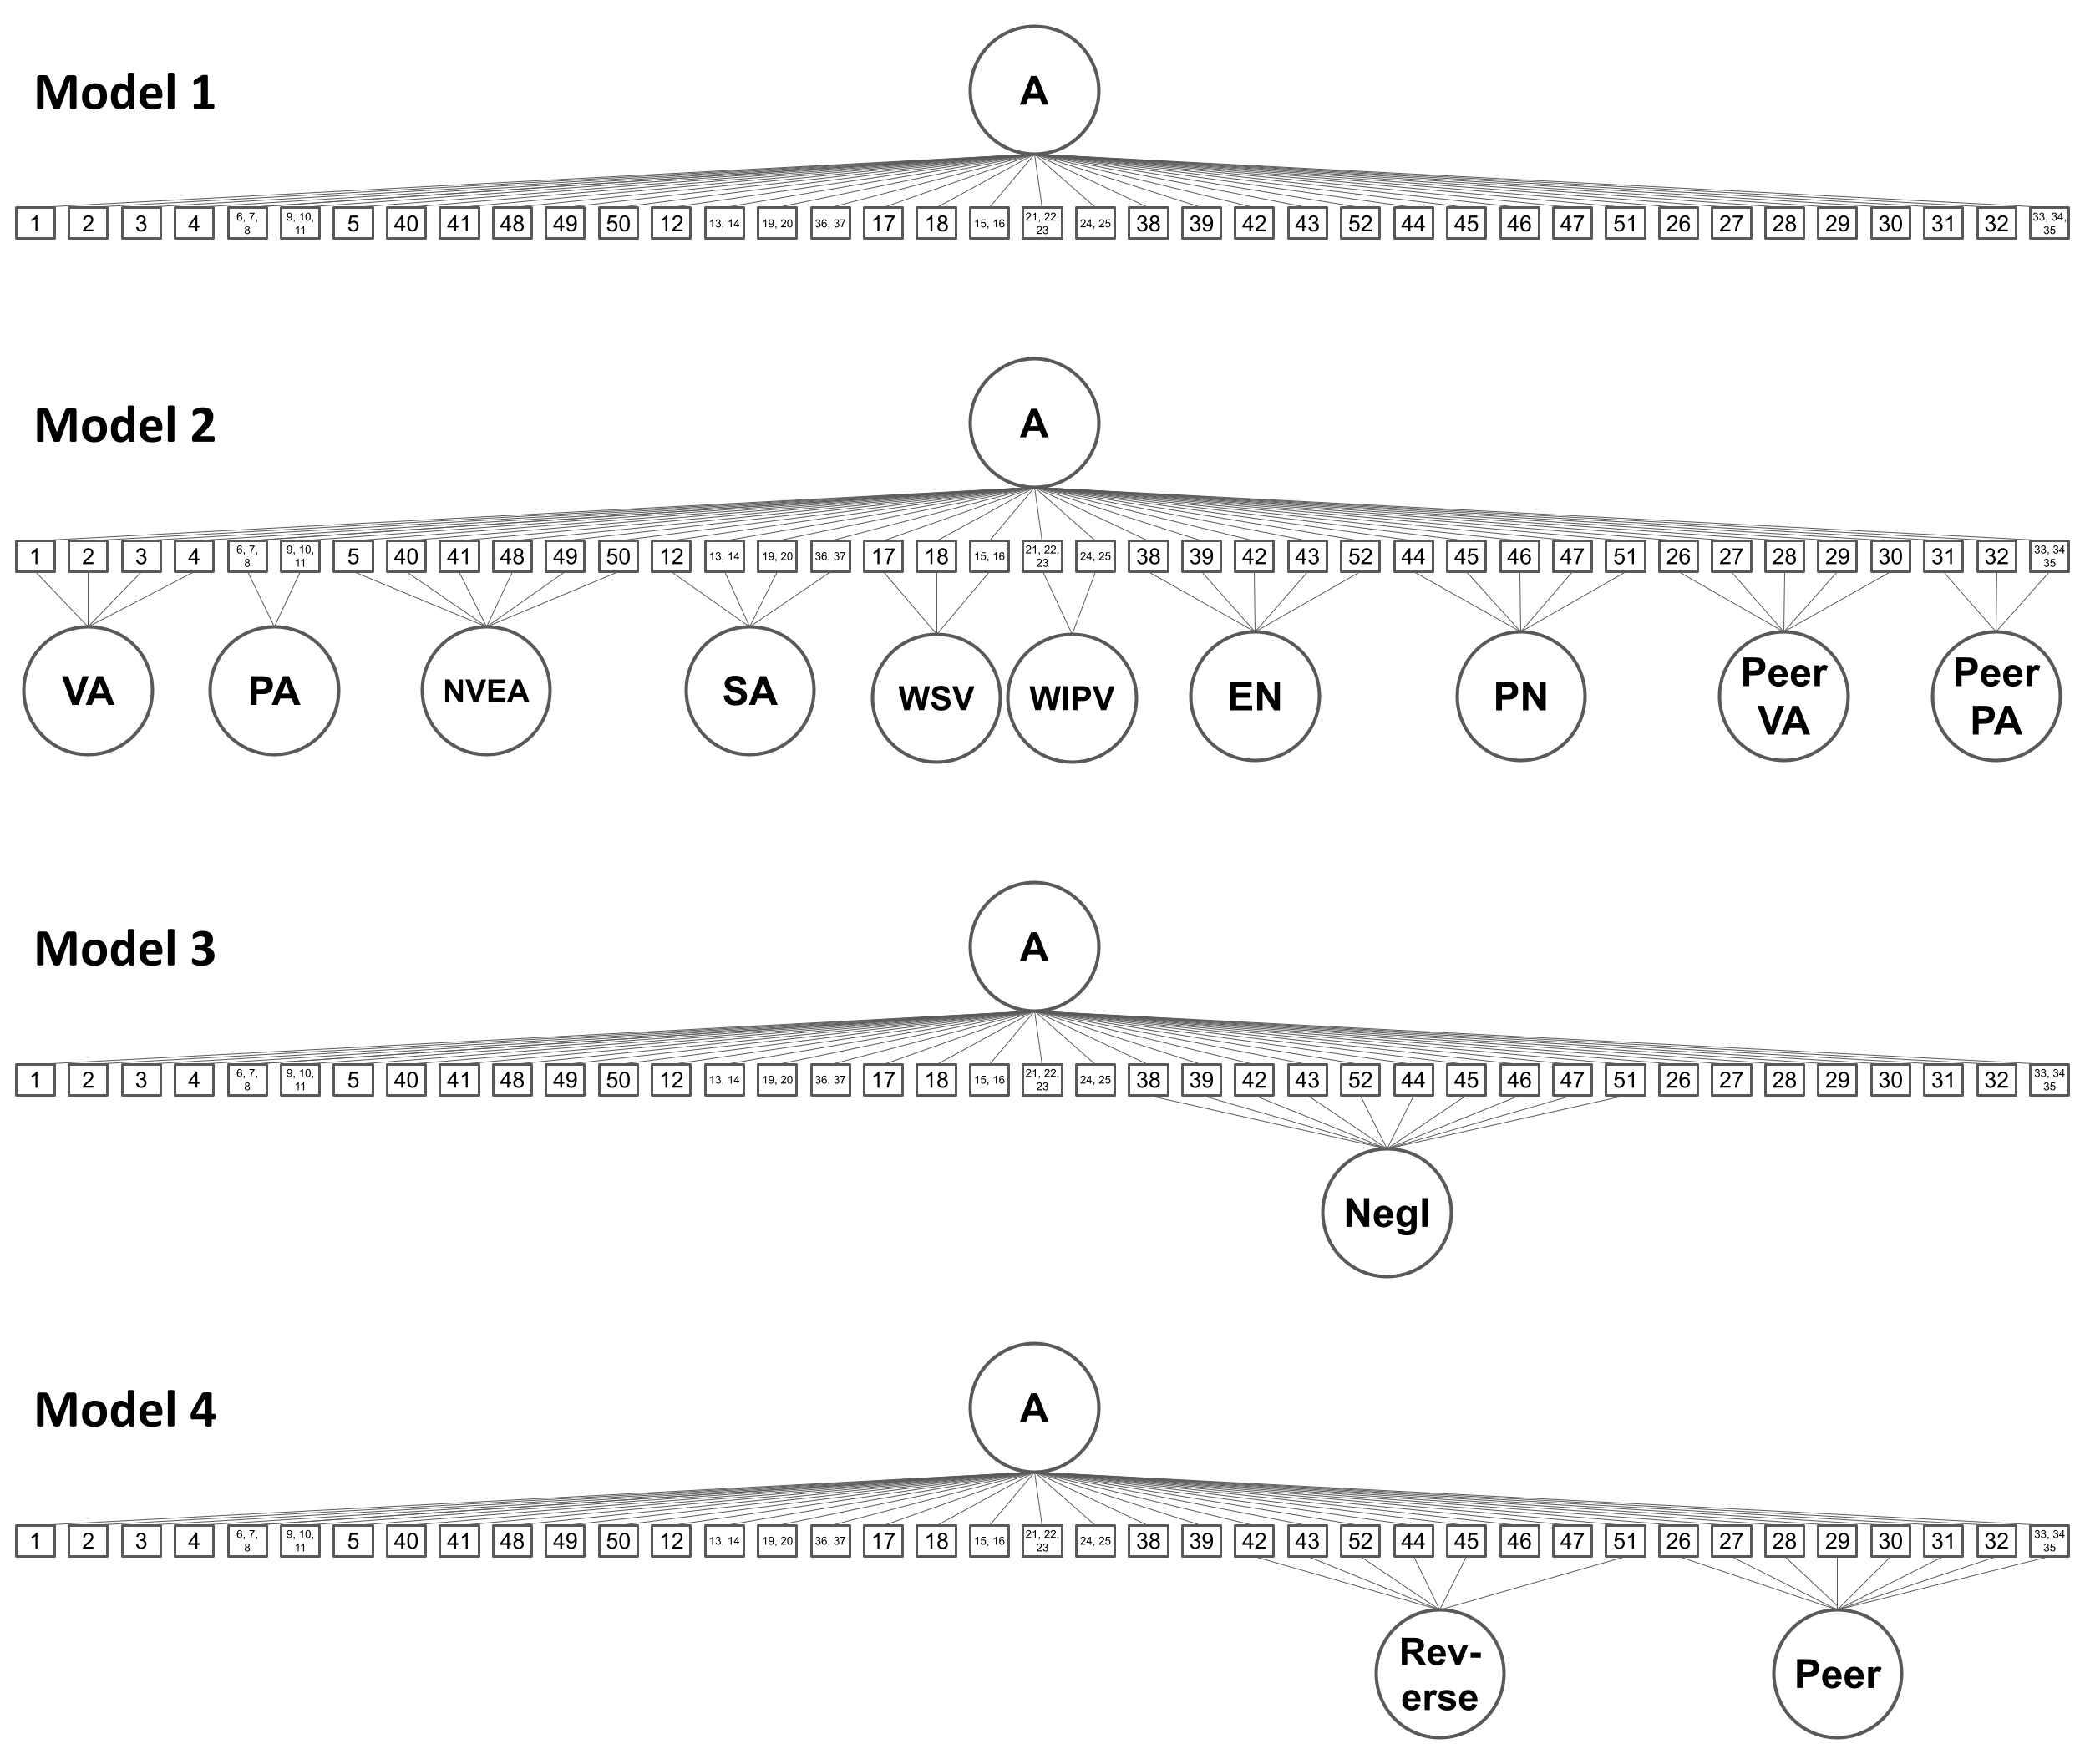
\includegraphics[width=1.1\textwidth,center]{figures/fig00.png}
    \caption{Caption}
    \label{fig:models}
\end{figure}

\begin{figure}
    \centering
    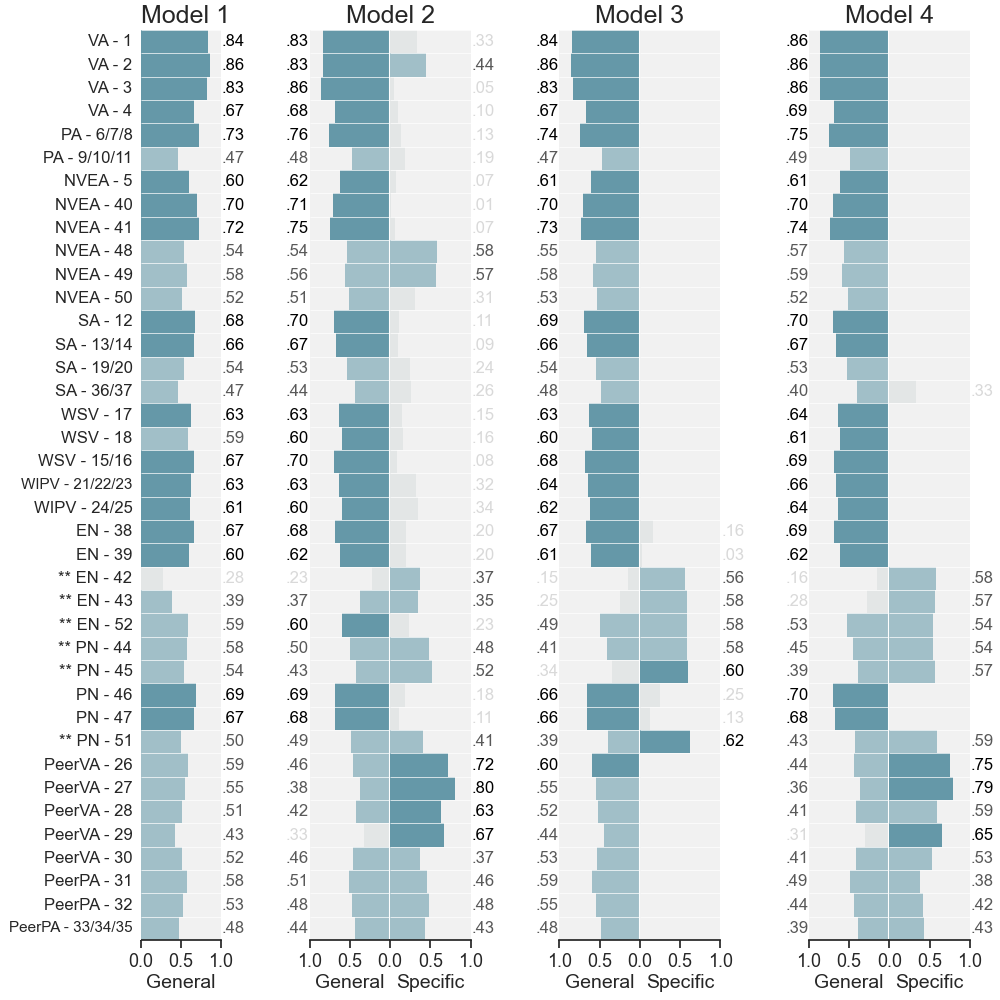
\includegraphics[width=1.1\textwidth,center]{figures/fig01.png}
    \caption{Standardized factor loadings from the four models estimated from the original sample. VA = verbal abuse; PA = physical abuse; NVEA = nonverbal emotional abuse; SA = sexual abuse; WSV = witnessing sibling vioence; WIPV = witnessing inter-parental violence; EN = emotional neglect; PN = physical neglect; PeerVA = peer verbal abuse; PeerPA = peer physical abuse. ** Reverse-scored items.}
    \label{fig:loadings_original}
\end{figure}

\begin{figure}
    \centering
    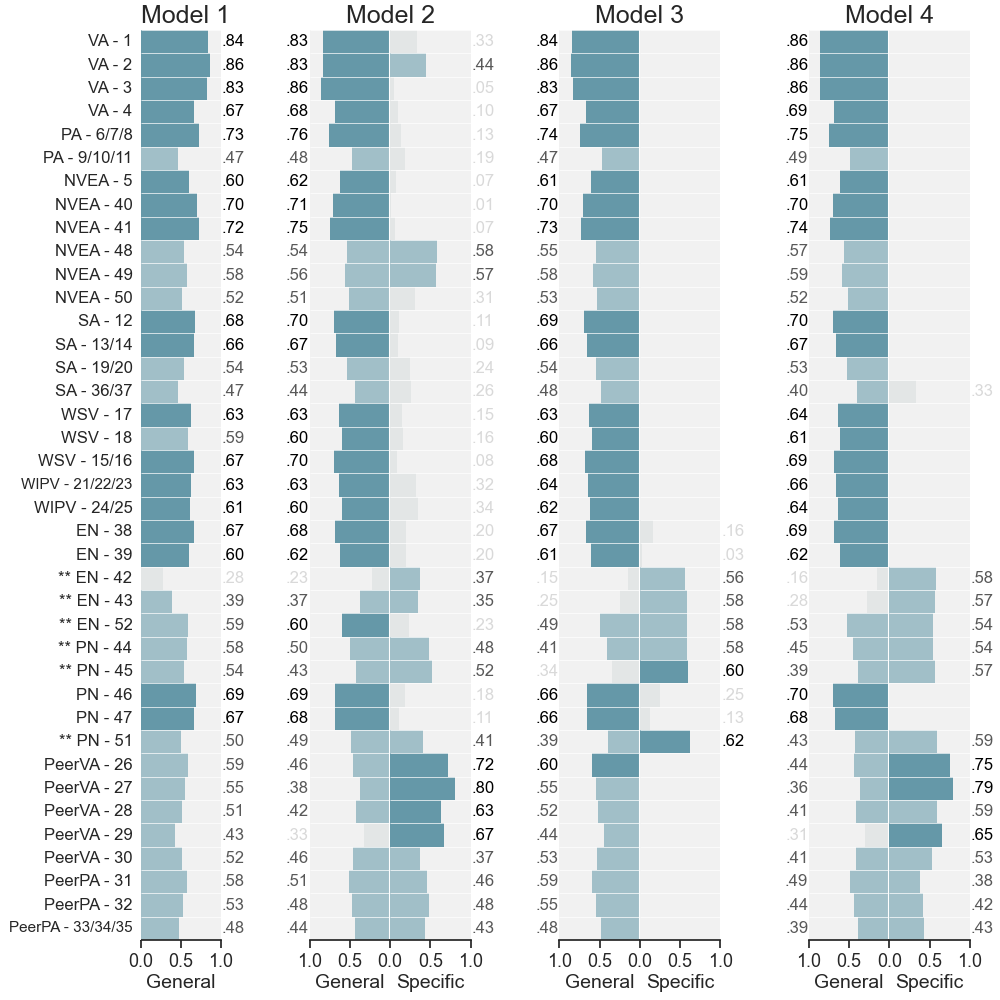
\includegraphics[width=1.1\textwidth,center]{figures/fig02.png}
    \caption{Standardized factor loadings from the four models estimated from the online sample. VA = verbal abuse; PA = physical abuse; NVEA = nonverbal emotional abuse; SA = sexual abuse; WSV = witnessing sibling vioence; WIPV = witnessing inter-parental violence; EN = emotional neglect; PN = physical neglect; PeerVA = peer verbal abuse; PeerPA = peer physical abuse. ** Reverse-scored items.}
    \label{fig:loadings_online}
\end{figure}

\begin{figure}
    \centering
    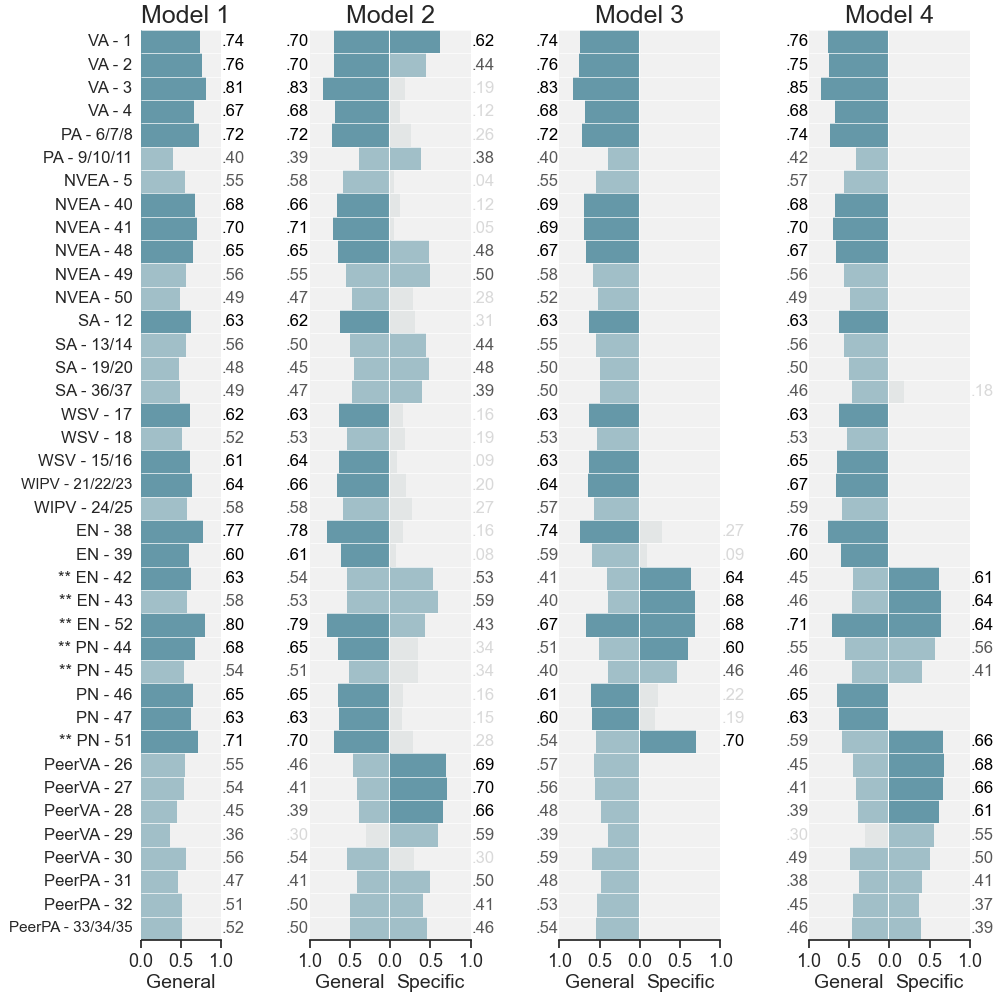
\includegraphics[width=1\textwidth,center]{figures/fig03.png}
    \caption{Caption}
    \label{fig:efa}
\end{figure}

\end{document}
